\section{Implementation}
\label{sec:implementation}

\subsection{Smart Contract Architecture}

EVMAuth's implementation follows a modular composition pattern where independent base contracts provide orthogonal features that combine into a unified authorization system. This architecture enables code reuse, simplifies testing, and allows selective feature composition for specialized deployments.

\textbf{Modular Inheritance Design.} The system consists of three architectural layers: (1) \textbf{Base Contracts} implement single-responsibility primitives (access control, token enumeration, ephemeral tokens, purchasing, transfer control), (2) \textbf{EVMAuth Core} composes all base contracts into a unified interface with coordinated configuration management, and (3) \textbf{Token Standard Implementations} (EVMAuth1155, EVMAuth6909) integrate token standard semantics with EVMAuth primitives. Figure~\ref{fig:contract-hierarchy} illustrates the complete inheritance structure.

Each base contract uses EIP-7201~\cite{erc7201} namespaced storage to prevent collisions in the proxy upgrade pattern. For example, \texttt{TokenPurchasable} stores its treasury address and pricing mappings at storage slot \texttt{keccak256("tokenpurchasable.storage.TokenPurchasable") \& \~{}0xFF}, ensuring isolation from other contract state even when multiple contracts inherit from the same base.

\textbf{Composition Pattern Benefits.} The modular design provides several advantages over monolithic contracts: (1) \textbf{Independent testing}---each base contract has isolated unit tests verifying single-responsibility behavior, (2) \textbf{Gas optimization}---unused features can be excluded in specialized deployments, (3) \textbf{Upgradeability}---individual primitives can be modified without rewriting the entire system, and (4) \textbf{Code clarity}---concerns are separated into well-defined boundaries (e.g., \texttt{TokenAccessControl} handles all role management, \texttt{TokenEphemeral} handles all TTL logic).

\begin{figure}[t]
\centering
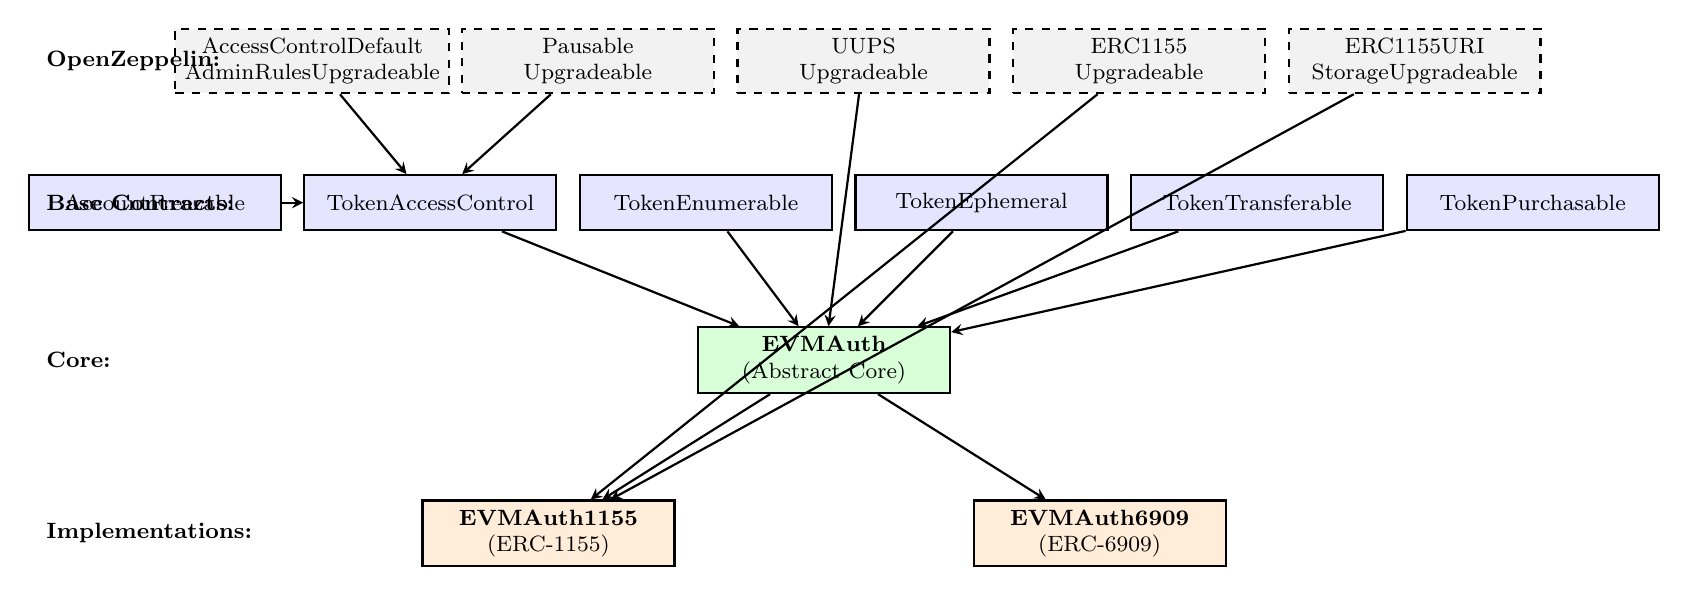
\begin{tikzpicture}[
    base/.style={rectangle, draw, thick, minimum width=3.2cm, minimum height=0.7cm, align=center, fill=blue!10, font=\footnotesize},
    core/.style={rectangle, draw, thick, minimum width=3.2cm, minimum height=0.7cm, align=center, fill=green!15, font=\footnotesize},
    impl/.style={rectangle, draw, thick, minimum width=3.2cm, minimum height=0.7cm, align=center, fill=orange!15, font=\footnotesize},
    oz/.style={rectangle, draw, thick, dashed, minimum width=3.2cm, minimum height=0.7cm, align=center, fill=gray!10, font=\footnotesize},
    arrow/.style={->,>=stealth,thick}
]

% OpenZeppelin Base Contracts (Top Layer - Dashed)
\node[oz] (ozaccess) at (0,6) {AccessControlDefault\\AdminRulesUpgradeable};
\node[oz] (ozpause) at (3.5,6) {Pausable\\Upgradeable};
\node[oz] (ozuups) at (7,6) {UUPS\\Upgradeable};
\node[oz] (oz1155) at (10.5,6) {ERC1155\\Upgradeable};
\node[oz] (oz1155uri) at (14,6) {ERC1155URI\\StorageUpgradeable};

% Base Contracts Layer (Second Layer)
\node[base] (accfreeze) at (-2,4.2) {AccountFreezable};
\node[base] (acccontrol) at (1.5,4.2) {TokenAccessControl};
\node[base] (enumerate) at (5,4.2) {TokenEnumerable};
\node[base] (ephemeral) at (8.5,4.2) {TokenEphemeral};
\node[base] (transfer) at (12,4.2) {TokenTransferable};
\node[base] (purchase) at (15.5,4.2) {TokenPurchasable};

% Core Layer (Third Layer)
\node[core] (evmauth) at (6.5,2.2) {\textbf{EVMAuth}\\(Abstract Core)};

% Implementation Layer (Bottom Layer)
\node[impl] (evm1155) at (3,0) {\textbf{EVMAuth1155}\\(ERC-1155)};
\node[impl] (evm6909) at (10,0) {\textbf{EVMAuth6909}\\(ERC-6909)};

% Inheritance Arrows - OpenZeppelin to Base Contracts
\draw[arrow] (ozaccess) -- (acccontrol);
\draw[arrow] (ozpause) -- (acccontrol);
\draw[arrow] (accfreeze) -- (acccontrol);

% Inheritance Arrows - Base Contracts to EVMAuth Core
\draw[arrow] (acccontrol) -- (evmauth);
\draw[arrow] (enumerate) -- (evmauth);
\draw[arrow] (ephemeral) -- (evmauth);
\draw[arrow] (transfer) -- (evmauth);
\draw[arrow] (purchase) -- (evmauth);
\draw[arrow] (ozuups) -- (evmauth);

% Inheritance Arrows - EVMAuth to Implementations
\draw[arrow] (evmauth) -- (evm1155);
\draw[arrow] (evmauth) -- (evm6909);

% Inheritance Arrows - OpenZeppelin to ERC-1155 Implementation
\draw[arrow] (oz1155) -- (evm1155);
\draw[arrow] (oz1155uri) -- (evm1155);

% Layer Labels
\node[anchor=west, font=\footnotesize\bfseries] at (-3.5,6) {OpenZeppelin:};
\node[anchor=west, font=\footnotesize\bfseries] at (-3.5,4.2) {Base Contracts:};
\node[anchor=west, font=\footnotesize\bfseries] at (-3.5,2.2) {Core:};
\node[anchor=west, font=\footnotesize\bfseries] at (-3.5,0) {Implementations:};

\end{tikzpicture}
\caption{EVMAuth contract inheritance hierarchy. Base contracts (blue) provide orthogonal authorization primitives. EVMAuth core (green) coordinates all primitives into a unified interface. Implementations (orange) integrate token standards (ERC-1155 or ERC-6909) with EVMAuth primitives. Dashed boxes represent OpenZeppelin dependencies.}
\label{fig:contract-hierarchy}
\end{figure}


\textbf{Coordination Layer.} The \texttt{EVMAuth} abstract contract provides the coordination layer between base contracts. It exposes the unified \texttt{EVMAuthTokenConfig} struct containing four fields (price, erc20Prices, ttl, transferable) and implements \texttt{createToken} and \texttt{updateToken} functions that atomically configure all base contracts. This ensures configuration consistency: setting a token's TTL to 30 days simultaneously configures \texttt{TokenEphemeral} for expiration tracking and prevents conflicting states across primitives.

\textbf{Token Standard Integration.} \texttt{EVMAuth1155} and \texttt{EVMAuth6909} extend \texttt{EVMAuth} with their respective token standards by implementing three integration points: (1) \texttt{\_update} hook to enforce transferability and account freezing during transfers, (2) \texttt{\_mintPurchasedTokens} to complete purchase transactions via standard minting functions, and (3) \texttt{balanceOf} override to integrate ephemeral token pruning with standard balance queries. Both implementations pass the same authorization test suite, verifying identical security properties despite different token semantics.

\subsection{Storage Optimization}

EVMAuth employs two storage optimization techniques to minimize gas costs while maintaining upgradeability: EIP-7201 namespaced storage for collision resistance and bounded arrays for ephemeral token records.

\textbf{EIP-7201 Namespaced Storage.} Upgradeable contracts using the UUPS proxy pattern face storage collision risks when adding new state variables in upgraded implementations. Traditional solutions (storage gaps, append-only layouts) are fragile and error-prone. EIP-7201~\cite{erc7201} solves this by computing deterministic storage slots from unique namespace strings. Each base contract defines a storage struct and computes its slot as: \texttt{keccak256(abi.encode(uint256(keccak256("namespace")) - 1)) \& \~{}bytes32(uint256(0xff))}. The subtraction by 1 and bitwise AND ensure the slot is outside the standard storage layout range, preventing accidental overwrites.

For example, \texttt{TokenPurchasable} declares:
\begin{lstlisting}[language=Solidity,basicstyle=\ttfamily\footnotesize]
struct TokenPurchasableStorage {
    address payable treasury;
    mapping(uint256 => uint256) nativePrices;
    mapping(uint256 => mapping(address => uint256)) erc20Prices;
    mapping(uint256 => address[]) erc20TokensAccepted;
}
bytes32 private constant TokenPurchasableStorageLocation =
    0x54c84cf2875b53587e3bd1a41cdb4ae126fe9184d0b1bd9183d4f9005d2ff600;
\end{lstlisting}

All state access occurs through \texttt{\_getTokenPurchasableStorage()}, which retrieves the storage pointer via inline assembly. This pattern prevents accidental direct storage access and makes collisions cryptographically improbable (probability $< 2^{-128}$ for random namespace strings).

\textbf{Bounded Arrays for Balance Records.} The time-bucketed balance records algorithm detailed in our previous work~\cite{tbbr} stores ephemeral token balances as arrays of timestamped records. Without bounds, malicious actors could create unbounded arrays through repeated small transfers, causing denial-of-service via out-of-gas errors during balance queries or transfers. EVMAuth enforces a maximum of $k+1$ records per account per token type, where $k$ is configurable per deployment (default: 100).

When a new record would exceed the limit, the algorithm drops the oldest bucket:
\begin{lstlisting}[language=Solidity,basicstyle=\ttfamily\footnotesize]
if (records.length >= _maxBalanceRecords()) {
    uint256 oldestBalance = records[0].balance;
    for (uint256 i = 1; i < records.length; i++) {
        records[i - 1] = records[i];
    }
    records.pop();
    return oldestBalance; // Lost due to fragmentation
}
\end{lstlisting}

This trades storage for predictable gas costs: worst-case transfer operations require $O(k^2)$ gas for splitting balances across full record sets, but storage per account remains constant. Section~\ref{sec:evaluation} quantifies this trade-off with $k=100$ and 30-day TTL, showing 11M gas worst-case transfers but bounded storage of 3.2KB per account.

\textbf{Storage Layout Verification.} OpenZeppelin's Foundry Upgrades plugin~\cite{openzeppelin} validates storage layouts during deployment, detecting accidental collisions, unsafe type changes, or deleted variables. The plugin compares current and upgraded contract ASTs, failing deployment if incompatible changes are detected. This automated verification prevents an entire class of upgrade-related vulnerabilities.

\subsection{Security Measures}

EVMAuth implements defense-in-depth security through four mechanisms: reentrancy protection, emergency pause functionality, role-based access control with least privilege, and time-delayed admin transfers.

\textbf{Reentrancy Protection.} Purchase functions transfer native currency or ERC-20 tokens to the treasury before minting authorization tokens. Without reentrancy protection, malicious treasury contracts could re-enter \texttt{purchase} during the treasury transfer, potentially minting tokens without payment or double-spending allowances. EVMAuth uses OpenZeppelin's \texttt{ReentrancyGuardTransientUpgradeable}~\cite{openzeppelin}, which leverages transient storage (EIP-1153) to track reentrant calls with significantly lower gas costs than persistent storage locks.

The transient reentrancy guard sets a lock flag in transient storage (5K gas) rather than persistent storage (20K gas), saving 15K gas per protected function call. The lock automatically resets at transaction end without requiring explicit cleanup, preventing the stuck-lock vulnerability of traditional reentrancy guards where failed transactions leave locks engaged.

\textbf{Pausability for Emergencies.} The \texttt{ACCESS\_MANAGER\_ROLE} can invoke \texttt{pause()} to immediately halt all token operations (purchases, transfers, minting) while preserving read-only functions (balance queries, configuration retrieval). This enables rapid response to detected vulnerabilities, oracle failures, or economic attacks without requiring emergency upgrades. For example, if an external ERC-20 payment token is compromised, pausing prevents attackers from purchasing authorization tokens with worthless assets while administrators analyze the situation.

Pausing affects state-modifying operations through the \texttt{whenNotPaused} modifier but explicitly excludes:
\begin{itemize}
\item Balance queries (\texttt{balanceOf}) for API authorization checks
\item Configuration retrieval (\texttt{tokenConfig}) for client applications
\item Administrative functions (role management, unpausing)
\item Balance record pruning for storage cleanup
\end{itemize}

This selective pausing ensures API authorization continues functioning (denying access for insufficient balances) even while the contract is paused, preventing service outages while addressing security incidents.

\textbf{Role Separation and Least Privilege.} EVMAuth defines six specialized roles beyond the default admin, each controlling orthogonal operations:

\begin{itemize}
\item \textbf{UPGRADE\_MANAGER\_ROLE}: Authorizes contract upgrades via UUPS proxy pattern. Separated from admin to enable cold storage of upgrade keys while keeping admin keys accessible for operational tasks.

\item \textbf{ACCESS\_MANAGER\_ROLE}: Controls pause/unpause and account freezing. Enables instant revocation without requiring treasury keys or token manager permissions.

\item \textbf{TOKEN\_MANAGER\_ROLE}: Creates and configures token types. Isolated from minting to prevent unauthorized token issuance while allowing price/TTL updates.

\item \textbf{MINTER\_ROLE}: Mints tokens to accounts. Granted to automated purchase contracts while denying them configuration or freezing capabilities.

\item \textbf{BURNER\_ROLE}: Burns tokens from accounts. Used for refunds or forced revocation, separated from minting to prevent combined mint+burn exploits.

\item \textbf{TREASURER\_ROLE}: Updates treasury address. Isolated to prevent attackers with other roles from redirecting revenue.
\end{itemize}

This separation follows the principle of least privilege: each operational concern (financial, technical, security) can be managed by specialized keys or multi-signature wallets. A compromised minter key cannot modify pricing, a compromised treasurer key cannot freeze accounts, and a compromised token manager cannot upgrade the contract.

\textbf{Time-Delayed Admin Transfers.} The default admin role uses OpenZeppelin's \texttt{AccessControlDefaultAdminRules}~\cite{openzeppelin}, which enforces a configurable delay (default: 2 days) between proposing and executing admin transfers. When \texttt{beginDefaultAdminTransfer(newAdmin)} is called, the transfer enters a pending state:

\begin{lstlisting}[language=Solidity,basicstyle=\ttfamily\footnotesize]
function beginDefaultAdminTransfer(address newAdmin)
    public
    onlyRole(DEFAULT_ADMIN_ROLE)
{
    _pendingDefaultAdmin = newAdmin;
    _pendingDefaultAdminSchedule = block.timestamp + delay();
    emit DefaultAdminTransferScheduled(newAdmin, _pendingDefaultAdminSchedule);
}
\end{lstlisting}

After the delay elapses, either party can finalize the transfer via \texttt{acceptDefaultAdminTransfer()}. This provides a detection window: monitoring systems can observe \texttt{DefaultAdminTransferScheduled} events, alerting operators to suspicious transfers. If an attacker compromises the admin key and initiates a transfer, legitimate operators have 2 days to revoke roles, pause the contract, or cancel the transfer before it executes.

The delay applies only to admin transfers, not other role grants, enabling rapid response to operational needs while protecting against takeover attacks. The current admin can cancel pending transfers at any time via \texttt{cancelDefaultAdminTransfer()}, providing an escape mechanism if a proposed transfer is detected as malicious.

\subsection{Deployment Considerations}

Deploying EVMAuth requires balancing gas costs, contract size constraints, and multi-chain compatibility.

\textbf{Gas Costs by Operation.} Table~\ref{tab:operation-costs} summarizes gas consumption for common operations across both implementations. Deployment costs dominate initial expenses: 5.4M gas for EVMAuth1155 (\$54 at 50 gwei, \$2,000/ETH) and 4.9M gas for EVMAuth6909 (\$49). Operational costs vary by complexity: configuration updates (14K-20K gas) are cheap, while ephemeral token transfers with full record sets can reach 11M gas in worst-case scenarios.

Services can optimize gas costs through: (1) using soulbound tokens to avoid transfer complexity entirely, (2) batching operations (ERC-1155 batch transfers save 30\% compared to sequential transfers), (3) periodic pruning of expired balance records to reduce fragmentation, and (4) selecting appropriate $k$ values based on expected transfer frequency (higher $k$ trades storage for cheaper transfers).

\textbf{Contract Size Constraints.} EVM contracts are limited to 24,576 bytes (EIP-170). EVMAuth1155 approaches this limit at 24,516 bytes (60 bytes margin), while EVMAuth6909 has 2,329 bytes of headroom. Both implementations required careful optimization:

\begin{itemize}
\item \textbf{Compiler optimization}: Solidity optimizer runs set to 200 optimize for execution costs while managing deployment size. Higher runs (e.g., 10,000) reduce execution gas but increase deployment size beyond the limit.

\item \textbf{Library extraction}: Shared logic moved to libraries (e.g., OpenZeppelin's SafeERC20) reduces deployment size at the cost of external calls (100 gas overhead).

\item \textbf{Error messages}: Custom errors (e.g., \texttt{error AccountFrozen(address)}) replace revert strings, saving 2-3 bytes per error while maintaining debuggability.

\item \textbf{Modifier inlining}: Frequently used modifiers are manually inlined in critical paths to avoid function call overhead at the cost of code duplication.
\end{itemize}

Future extensions may require removing features (e.g., batch operations, metadata storage) or splitting functionality across multiple contracts. EVMAuth6909's larger margin provides more flexibility for feature additions.

\textbf{Multi-Chain Deployment Strategy.} EVMAuth is EVM-compatible, supporting deployment to Ethereum, Base, Polygon, Arbitrum, Optimism, and other L1/L2 networks. Deployment strategy varies by chain characteristics:

\begin{itemize}
\item \textbf{High-cost chains} (Ethereum mainnet): Deploy EVMAuth6909 for lower deployment costs. Use soulbound tokens to minimize transfer gas. Consider deploying with higher $k$ values (e.g., 200) to reduce transfer costs at the expense of storage.

\item \textbf{Low-cost chains} (Base, Polygon): Deploy EVMAuth1155 for ecosystem compatibility. Batch operations and marketplace integration outweigh marginal gas savings.

\item \textbf{Private/consortium chains}: Deploy with custom optimizations. Remove purchase functionality if payments are handled off-chain. Adjust $k$ and TTL parameters for specific use cases.
\end{itemize}

All deployments use the UUPS proxy pattern, enabling upgrades without redeploying dependent infrastructure. Proxy addresses remain constant across upgrades, ensuring API integrations and client applications continue functioning without configuration changes. The OpenZeppelin Foundry Upgrades plugin validates upgrade safety during deployment, preventing storage collisions and unsafe type changes.
